\documentclass[conference]{IEEEtran}

% --------------------------------------------
% Packages
% --------------------------------------------

\usepackage{graphicx}
\usepackage{amsmath}
\usepackage{cite}
\usepackage{booktabs}
\usepackage{float}
\usepackage{caption}
\usepackage{subcaption}

% --------------------------------------------
% Document
% --------------------------------------------

\begin{document}

% --------------------------------------------
% Title
% --------------------------------------------

\title{
Effect of Hydrogen Enrichment on Laminar Flame Speed and Adiabatic Flame Temperature of Premixed Methane-Air Flames Using Cantera
}

% --------------------------------------------
% Authors
% --------------------------------------------

\author{

\IEEEauthorblockN{
Omkar Das,
Suyash Trivedi,
Rutrank Tandon,
Uday Chaudhary,
Utkarsh Ashish Pandey
}

\IEEEauthorblockA{
Department of Mechanical Engineering\\
R. V. College of Engineering\\
Bengaluru, India\\
USN: 1RV23ME077, 1RV23ME115, 1RV23ME092, 1RV23ME119, 1RV23ME120\\
Email: omkardas.me23@rvce.edu.in
}

}

\maketitle

% --------------------------------------------
% Abstract
% --------------------------------------------

\begin{abstract}

Hydrogen enrichment of methane-air mixtures has gained significant attention due to its potential in improving combustion efficiency and reducing carbon emissions in modern energy systems. In this work, a computational investigation of premixed methane-hydrogen-air combustion was performed using the Cantera Python package and the GRI-Mech 3.0 chemical kinetics mechanism. A one-dimensional freely propagating laminar flame model was employed to study the influence of hydrogen addition on laminar flame speed and adiabatic flame temperature. Hydrogen fractions ranging from 0\% to 40\% and equivalence ratios from 0.6 to 1.4 were analyzed under atmospheric pressure and an inlet temperature of 300 K. The results indicate that hydrogen enrichment significantly increases laminar flame speed while causing a moderate increase in adiabatic flame temperature. Maximum flame speeds were observed near stoichiometric conditions. The obtained trends are consistent with established combustion literature and demonstrate the importance of hydrogen blending in future low-carbon combustion systems.

\end{abstract}

% --------------------------------------------
% Keywords
% --------------------------------------------

\begin{IEEEkeywords}

Hydrogen enrichment, methane combustion, laminar flame speed, adiabatic flame temperature, Cantera, GRI-Mech 3.0

\end{IEEEkeywords}

% --------------------------------------------
% Introduction
% --------------------------------------------

\section{Introduction}

Hydrogen-enriched methane combustion has emerged as a promising approach for reducing carbon emissions while maintaining high combustion efficiency in industrial combustion systems and gas turbines \cite{Garcia_2023,en14102834,Hermanns2007}. Hydrogen blending improves flame stability, increases laminar flame speed, and extends flammability limits due to the high diffusivity and reactivity of hydrogen molecules. Previous experimental and numerical investigations have demonstrated that hydrogen enrichment can significantly enhance combustion performance under lean operating conditions \cite{doi:10.1021/acsomega.1c01692,Garcia_2023}.

Laminar flame speed is one of the most fundamental properties of premixed combustion systems, as it governs flame propagation, combustion stability, flashback tendency, and pollutant formation \cite{doi:10.1021/acsomega.1c01692}. Similarly, adiabatic flame temperature plays an important role in determining combustion efficiency and thermal NO$_x$ formation.

Recent advances in computational combustion tools such as Cantera have enabled detailed numerical investigations of reacting flows using validated chemical kinetics mechanisms \cite{Marzouk_2023,Mao_2023}. Among the available detailed chemical kinetics mechanisms, GRI-Mech 3.0 remains one of the most widely used mechanisms for methane-air combustion simulations because of its balance between computational efficiency and predictive capability \cite{en14102834,Zhou2021-eq,GIMENOESCOBEDO201927123}. Reduced chemical mechanisms have also been developed in recent years to decrease computational cost while preserving combustion accuracy for methane-hydrogen mixtures \cite{Zhou2021-eq,GIMENOESCOBEDO201927123}.

In this study, the effect of hydrogen enrichment on premixed methane-air flames is numerically investigated using Cantera and GRI-Mech 3.0. The influence of hydrogen fraction and equivalence ratio on laminar flame speed and adiabatic flame temperature is analyzed under atmospheric conditions.

% --------------------------------------------
% Literature Review
% --------------------------------------------

\section{Literature Review}

Several experimental and computational investigations have examined the combustion behavior of methane-hydrogen fuel blends under varying operating conditions. Garcia et al. \cite{Garcia_2023} studied the effect of hydrogen addition on lean premixed methane flames and reported increased flame consumption speed under hydrogen enrichment conditions.

Paykani \cite{en14102834} compared multiple chemical kinetics mechanisms for methane-based fuel mixtures and concluded that GRI-Mech 3.0 provides reliable predictions for laminar flame speed and ignition delay behavior under engine-relevant conditions.

Luo et al. \cite{doi:10.1021/acsomega.1c01692} experimentally investigated lean methane-air laminar premixed flames and demonstrated the importance of equivalence ratio and temperature on combustion characteristics.

Recent computational combustion studies have also focused on reduced chemical mechanisms and computational efficiency improvements. Zhou et al. \cite{Zhou2021-eq} developed a reduced methane-hydrogen mechanism for engine-relevant combustion simulations, while Gimeno-Escobedo et al. \cite{GIMENOESCOBEDO201927123} proposed a reduced methane-hydrogen mechanism suitable for cooktop burner simulations.

Advanced computational platforms such as DeepFlame \cite{Mao_2023} have further expanded the capabilities of reacting flow simulations through high-performance numerical frameworks and machine learning assisted combustion modeling.

% --------------------------------------------
% Methodology
% --------------------------------------------

\section{Methodology}

\subsection{Computational Setup}

The simulations were performed using the Cantera Python package with the GRI-Mech 3.0 detailed chemical kinetics mechanism. Freely propagating one-dimensional premixed flames were solved using the \texttt{FreeFlame} solver.

The inlet temperature and pressure were fixed at 300 K and 1 atm respectively. Hydrogen enrichment levels of 0\%, 10\%, 20\%, 30\%, and 40\% were investigated.

\subsection{Equivalence Ratio}

The equivalence ratio is defined as:

\begin{equation}
\phi = \frac{(F/A)_{actual}}{(F/A)_{stoichiometric}}
\end{equation}

where $(F/A)$ represents the fuel-air ratio.

The equivalence ratio was varied from 0.6 to 1.4 in order to study lean, stoichiometric, and rich combustion conditions.

\subsection{Simulation Parameters}

\begin{table}[H]
\centering
\caption{Simulation Parameters}
\begin{tabular}{cc}
\toprule
Parameter & Value \\
\midrule
Pressure & 1 atm \\
Inlet Temperature & 300 K \\
Hydrogen Fraction & 0--40\% \\
Equivalence Ratio & 0.6--1.4 \\
Mechanism & GRI-Mech 3.0 \\
Solver & Cantera FreeFlame \\
\bottomrule
\end{tabular}
\end{table}

% --------------------------------------------
% Results
% --------------------------------------------

\section{Results and Discussion}

\subsection{Laminar Flame Speed}

Figure~\ref{fig:flame_speed} shows the variation of laminar flame speed with equivalence ratio for different hydrogen enrichment levels.

\begin{figure}[H]
\centering
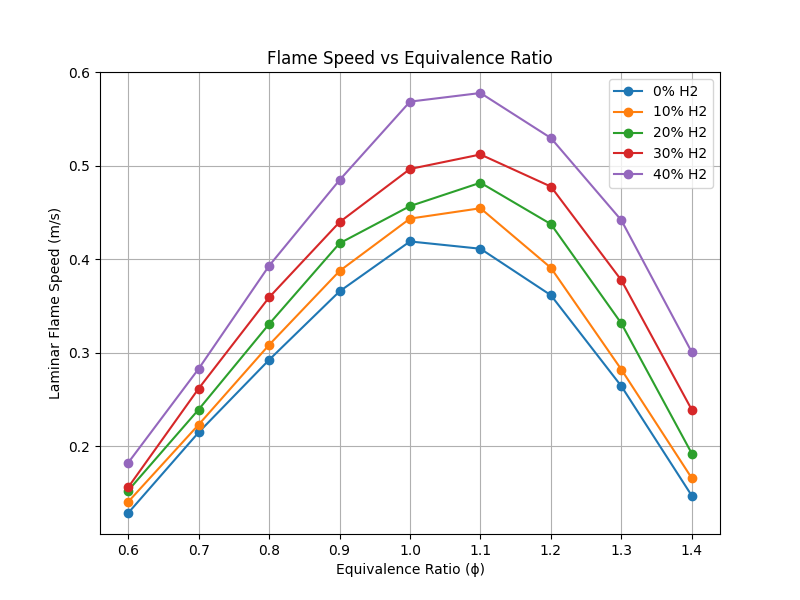
\includegraphics[width=0.48\textwidth]{figures/flame_speed.png}
\caption{Laminar flame speed variation with equivalence ratio for different hydrogen fractions.}
\label{fig:flame_speed}
\end{figure}

The results indicate that laminar flame speed increases significantly with hydrogen enrichment, which is consistent with previous experimental and numerical methane-hydrogen combustion studies reported in literature \cite{Garcia_2023,Hermanns2007,hesse2026physicsguidedlaminarflamespeed}. The maximum flame speed occurs near stoichiometric conditions ($\phi \approx 1.0 - 1.1$). Hydrogen addition enhances flame propagation due to increased diffusivity and chain branching reactions involving reactive radicals such as H, O, and OH.

\subsection{Adiabatic Flame Temperature}

Figure~\ref{fig:flame_temperature} illustrates the variation of adiabatic flame temperature with equivalence ratio.

\begin{figure}[H]
\centering
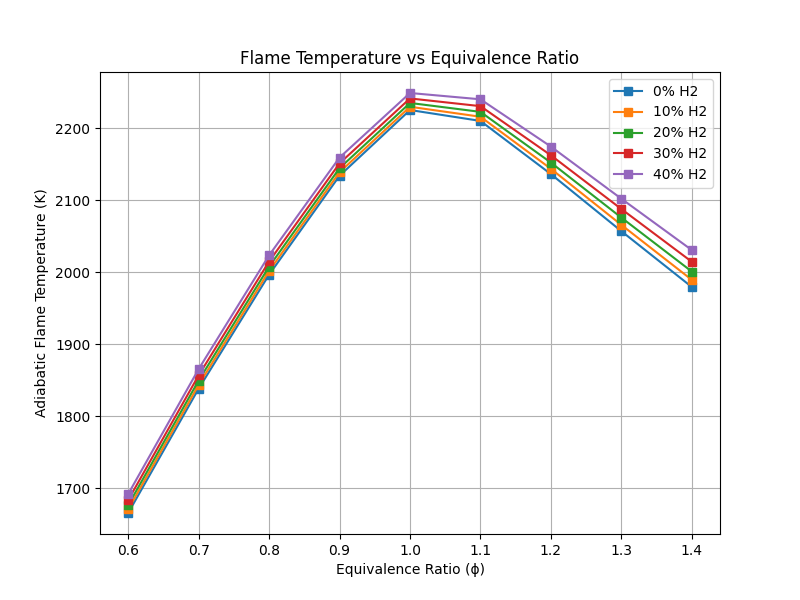
\includegraphics[width=0.48\textwidth]{figures/flame_temperature.png}
\caption{Adiabatic flame temperature variation with equivalence ratio for different hydrogen fractions.}
\label{fig:flame_temperature}
\end{figure}

The flame temperature reaches a maximum near stoichiometric combustion conditions and decreases under both lean and rich mixtures. Hydrogen enrichment causes a moderate increase in flame temperature due to enhanced combustion reactivity and faster radical formation kinetics. Similar adiabatic flame temperature trends have been reported in previous Cantera-based combustion investigations \cite{Marzouk_2023}.

\subsection{Discussion}

The computational results obtained in this work are consistent with previous methane-hydrogen combustion studies reported in literature \cite{hesse2026physicsguidedlaminarflamespeed,Garcia_2023}. The increase in flame speed with hydrogen enrichment improves combustion stability and enables ultra-lean combustion operation. Hydrogen enrichment also extends flammability limits and enhances combustion reactivity under lean conditions. However, higher flame speeds may increase flashback risk and combustor design complexity in practical gas turbine and industrial burner applications.

% --------------------------------------------
% Conclusion
% --------------------------------------------

\section{Conclusion}

A computational study of hydrogen-enriched premixed methane-air combustion was performed using Cantera and the GRI-Mech 3.0 mechanism. The effect of hydrogen fraction and equivalence ratio on laminar flame speed and adiabatic flame temperature was analyzed.

The results demonstrate that hydrogen enrichment significantly increases laminar flame speed while moderately increasing adiabatic flame temperature. Peak combustion performance was observed near stoichiometric conditions. The study highlights the potential of hydrogen blending in future low-carbon combustion systems while emphasizing the importance of flame stability and flashback considerations.

Future work may include NO$_x$ prediction, elevated pressure simulations, and detailed species transport analysis for hydrogen-enriched combustion systems.

% --------------------------------------------
% References
% --------------------------------------------

\nocite{*}
\bibliographystyle{IEEEtran}
\bibliography{references}

\end{document}